\chapter{Examples}

The \eTrice{} examples can be installed using the new wizard.

Choose File > New > Other (or Ctrl-N), open category "eTrice".
There are examples for C and for Java. Each of them consists of a single
Eclipse project that contains several examples which are described
in the next sections.
Select the desired one, click Next and Finish and you are ready to go.

As already mentioned each example project contains several examples.
Each of them comes with a room model, a mapping model a launch configuration
for the code generation and a launch configuration to run the compiled example.

\section{The C examples project}

This example project \texttt{org.eclipse.etrice.examples.c} illustrates
a simplified traffic light control.
It actually consists of four different steps of increasing
complexity that can be generated and
built one by one (but not in parallel).

Most of the classes are contained in a common ROOM model
\texttt{model/TrafficLight/TrafficLight.room} that also shows
how ROOM classes can form a library and used as building blocks for several systems.
Also the physical model is shared by all steps of this example.

Contained in the example you will find a little Java GUI that some of the
example use to simulate a real traffic light. The GUI is contacted
using TCP/IP ports 4441 and subsequent. The protocol used on the TCP/IP
socket connection is a simple text protocol with commands for the lights.
Three of the example steps make use of this simulator GUI. They
also contain a launch configuration for it.

\textbf{Note:} Before compiling and linking a new step of the example
the project should be cleaned to avoid duplicate symbols due to
artifacts from the previous build.

\subsection{Traffic light - step 1}

The main ROOM model and the mapping model of this example is contained
in \texttt{org.eclipse.etrice.examples.c/model/TrafficLight\_step1}.
It also contains launch configurations for the code generation and for
running the application.

\subsubsection{Purpose}

This example illustrates how a single actor can be tested against a test harness.

\subsubsection{Details}

A \texttt{PedestrianTrafficLightController} is an actor that controls a traffic light
consisting of a traffic light with red, yellow and green for the cars, a second
traffic light with just red and green and a request button for the pedestrians.

The controller has two ports, \texttt{fct} and \texttt{tlInterface}. The first
one uses a protocol \texttt{PTrafficLightController} that offers the high level
commands \texttt{standby}, \texttt{start} and \texttt{stop}. The second one
uses a conjugated protocol \texttt{PTrafficLightInterface} which controls
each of the lights separately.

The test harness \texttt{TrafficLightControllerTestHarness} is connected to
both ports and drives the test in several steps.

To run the test first generate the code using \texttt{gen\_TrafficLight\_step1.launch},
then compile and link it (using the CDTbuild). Since this step doesn't use a GUI
you can just start the application using \texttt{run\_TrafficLight\_step1.launch}.

\subsubsection{Noteworthy}

\begin{itemize}
\item usage of a ROOM model as library for several systems
\item creation of a test harness for an actor 
\end{itemize}

\subsection{Traffic light - step 2}

The main ROOM model and the mapping model of this example is contained
in \texttt{org.eclipse.etrice.examples.c/model/TrafficLight\_step2}.
It also contains launch configurations for the code generation, for
launching the simulator GUI and for
running the application.

\subsubsection{Purpose}

This example shows the control of a single block of traffic lights
containing a car light and a light for the pedestrians.
It illustrates how a stack of abstraction levels is used to conveniently
divide the problem into relatively simple parts.

\subsubsection{Details}

The 4 levels of this application starts with a
\texttt{TrafficLightHeadquarters} on the
top. It controls the global operating mode of the traffic light block.
The test harness \texttt{TrafficLightControllerTestHarness} is connected to
both ports and drives the test in several steps.

On the next level we have a \texttt{PedestrianTrafficLightController} which
offers some very general commands like \texttt{start}, \texttt{stop} and \texttt{standby}.

On the second level we find an actor \texttt{PTrafficLightInterface}
that offers basic traffic light control in the form of switching the state
of each single light separately.

On the base level we have an actor handling a TCP/IP socket
connection with a general text protocol.

To run the test first generate the code using \texttt{gen\_TrafficLight\_step2.launch},
then compile and link it (using the CDTbuild). Since this step uses a GUI with a
single block of lights
you'll have to launch the simulator using \texttt{run\_simulator\_1\_block.launch}.
Then you can just start the application using \texttt{run\_TrafficLight\_step2.launch}.

After going through a short initialization and standby phase the traffic
light goes into a mode of permanent green for cars.
After pressing the 'request' button in the simulator GUI the light switches
to red for cars and green for pedestrians and back to permanent green for cars.

\subsubsection{Noteworthy}

\begin{itemize}
\item use abstraction levels to break a problem into smaller pieces.
\end{itemize}

\subsection{Traffic light - step 3}

The main ROOM model and the mapping model of this example is contained
in \texttt{org.eclipse.etrice.examples.c/model/TrafficLight\_step3}.
It also contains launch configurations for the code generation, for
launching the simulator GUI and for
running the application.

\subsubsection{Purpose}

This example shows the control of two blocks of traffic lights
each containing a car light and a light for the pedestrians.
It uses a replicated stack of actors as introduced in step 2.

\subsubsection{Details}

The head quarters actor of this example controls two blocks of traffic
lights. It already has a replicated port which is now connected
to a doubled \texttt{PedestrianTrafficLightController}.
Of course the replication then has also to be applied to the other
levels of the stack introduced in step 2.

To run the test first generate the code using \texttt{gen\_TrafficLight\_step3.launch},
then compile and link it (using the CDTbuild). Since this step uses a GUI with a
two blocks of lights
you'll have to launch the simulator using \texttt{run\_simulator\_2\_blocks.launch}.
Then you can just start the application using \texttt{run\_TrafficLight\_step3.launch}.

\subsubsection{Noteworthy}

\begin{itemize}
\item use replication for multiple instances of the same.
\end{itemize}


\subsection{Traffic light - step 4}

The main ROOM model and the mapping model of this example is contained
in \texttt{org.eclipse.etrice.examples.c/model/TrafficLight\_step4}.
It also contains launch configurations for the code generation, for
launching the simulator GUI and for
running the application.

\subsubsection{Purpose}

This example shows the control of two blocks of traffic lights
each containing a car light and a light for the pedestrians.
It uses a container actor for the three lower levels of the stack
introduced in step 2. Then replication has to applied only to the
container actor which simplifies the task.

\subsubsection{Details}

The head quarters actor of this example controls two blocks of traffic
lights. It already has a replicated port which is now connected
to a doubled \texttt{TrafficLightControllerWithInfrastructure}.
The latter one 

\subsubsection{Noteworthy}

\begin{itemize}
\item use hierarchy to group levels functionality to reusable blocks.
\end{itemize}

\subsection{Features}

This project illustrates the various ways how replication can be exploited in
ROOM. Replication can be chosen for ports and for actor references.
The example enumerates a number of typical combinations of the two
possibilities.

\subsubsection{Purpose}

Five different ways to combine replicated ports and replicated actor references
are shown in this example.

Each of these combination consists of one ore more receivers and one or more
senders.

All five combinations are contained in the actor class \texttt{ExampleMultiplicity}.

\begin{itemize}
\item \texttt{sender1} and \texttt{receiver1} - a single sender and a single
receiver, both with plain ports, are connected.
\item \texttt{multiSender2} with a replication factor of 10 is connected to
\texttt{multiReceiver2} also with a replication factor of 10 - this is
equivalent to 10 single senders each of which is connected to one single out
of 10 receivers
\item \texttt{multiSender3} with a replication factor of 2 is connected to
\texttt{receiverMultiPort3} which has a port with replication factor 2
\item \texttt{multiSender4} with a replication factor of 10 is connected to
\texttt{multiReceiverMultiPort4} with a replicated port with cardinality 2
and replicated 5 times - this is equivalent to 5 receivers where each is connected
to two senders
\item \texttt{multiSender5} is connected to
\begin{itemize}
\item \texttt{receiver5} which is a simple receiver not using any replication
\item \texttt{multiReceiver5} which is a replicated receiver
\item \texttt{} which is not replicated but uses a replicated portreceiverMultiPort5
\item \texttt{multiReceiverMultiPort5} which is replicated and has replicated ports
\end{itemize}
So \texttt{multiSender5} is connected
\begin{itemize}
\item once to \texttt{receiver5}
\item three times to \texttt{multiReceiver5}
\item two times to \texttt{receiverMultiPort5} and
\item four times to \texttt{multiReceiverMultiPort5}
\end{itemize}
which totals to 10 (implicit) connections and matches the replication factor of
10 of \texttt{multiSender5}.
\end{itemize}

\subsubsection{Details}

The head quarters actor of this example controls two blocks of traffic
lights. It already has a replicated port which is now connected
to a doubled \texttt{TrafficLightControllerWithInfrastructure}.
The latter one 

\subsubsection{Noteworthy}

\begin{itemize}
\item use hierarchy to group levels of functionality to reusable blocks.
\end{itemize}

\section{The Java examples project}

The example project \texttt{org.eclipse.etrice.examples.java} currently contains
a number of examples that are all related to dynamic actors.

The examples can be generated and executed one by one but not several at the same
time. Inside the model folder there exists a sub folder for each example
containing all models and launch configurations for code generation and to
run the application.

\subsection{Dynamic Actors 1}

This example is contained in \texttt{model/dynamicactors1}.

\subsubsection{Purpose}

The example demonstrates the usage of an optional actor. It is shown that several actor classes
derived from the type of the optional actor reference can be optionally created in place
of the optional actor reference. Optional actor instances can also be destroyed
and another instance can be created in the free slot.

\subsubsection{Details}

The structure of this system is simple.

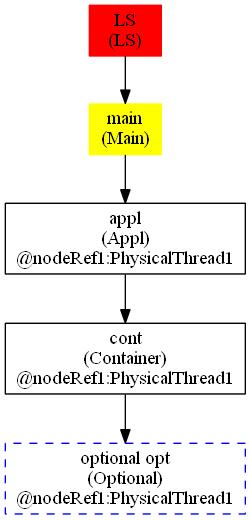
\includegraphics[scale=0.7]{images/039-DynAct1-Main_instanceTree.jpg}

However, this is only the initial system structure.
The leaf instance is just a place holder for an optional actor instance.
In this place an instance of a compatible type can be created at run time.
Compatible types are the type of the reference itself and all of its sub types as long as they are not abstract.
Together with the instance all of its contained instances will be created and all ports are connected.

This example demonstrates how an optional actor is created and destroyed and another one of another type
is created to hold the same place.

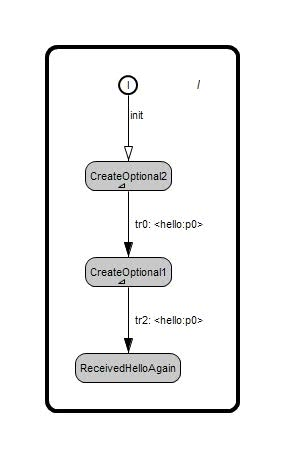
\includegraphics[scale=0.7]{images/039-DynAct1-Container_behavior.jpg}

When the example is executed the \texttt{Container} actor first dumps the instance tree to the console
(line 56 of the listing below).
Then it creates an instance of \texttt{Optional2} (line 57). Now that the \texttt{p0} port
of the container is connected a message \texttt{sayHello()} is sent to the newly created actor instance
and the instance tree is dumped a second time.
As soon as it receives the answer it prints it to the console. Then the optional actor is destroyed again
and another one, now of type \texttt{Optional1}, is created and once more \texttt{sayHello()} is sent.

\lstinputlisting[language=ROOM, firstnumber=36, firstline=36, lastline=73, caption=Container actor state machine]{../../../examples/org.eclipse.etrice.examples.java/model/dynamicactors1/DynAct1.room}

The console output of the running application starts with

\begin{verbatim}
***   T H E   B E G I N   ***
*** MainComponent /LS/main::init ***
type 'quit' to exit
before creation of Optional2
LS
  main
    RTSystemPort
    MessageService_MessageService_PhysicalThread1
      Dispatcher
      Queue
    ActorClass(className=Appl, instancePath=/LS/main/appl)
      port RTSystemPort
      ActorClass(className=Container, instancePath=/LS/main/appl/cont)
        port RTSystemPort
        port p0
        ScalarOptionalActorInterface(className=Optional, instancePath=/LS/main/appl/cont/opt)
          RTSystemPort
          port p0
    port RTSystemPort0
    port RTSystemPort1
\end{verbatim}

The \texttt{ScalarOptionalActorInterface(className=Optional, instancePath=/LS/main/appl/cont/opt)} is an object which is
responsible for the life cycle of the dynamic actor (including its contained instances) and for the mediation of the
port connections. It contains a replicated \texttt{RTSystemPort} which is used to trigger the initial transition and the
port \texttt{p0} of the interface of the \texttt{Optional} actor class.

After creation of \texttt{Optional2} the interesting part of the dumped tree is

\begin{verbatim}
        ScalarOptionalActorInterface(className=Optional, instancePath=/LS/main/appl/cont/opt)
          RTSystemPort
          port p0
          ActorClass(className=Optional2, instancePath=/LS/main/appl/cont/opt/opt)
            port RTSystemPort
            ActorClass(className=AC2, instancePath=/LS/main/appl/cont/opt/opt/sub2)
              port RTSystemPort
              ActorClass(className=AC3, instancePath=/LS/main/appl/cont/opt/opt/sub2/deep_sub)
                port RTSystemPort
                port p0
          port RTSystemPort0
          port RTSystemPort1
          port RTSystemPort2
\end{verbatim}

It can be seen that the sub tree corresponding to \texttt{Optional2} was inserted right below the
\texttt{ScalarOptionalActorInterface}.

After deletion of the optional actor the dumped instance tree looks exactly as in the beginning.

To illustrate the dynamic behavior of the system we can finally have a look at the generated
sequence diagram \ref{fig:dynact1_msc}. During the sub system initialization three actor
instances are created. Then the system is started and the \texttt{Container} actor dynamically creates
an instance of \texttt{Optional2}. This is indicated by the note on the life line of \texttt{/LS/main/appl/cont}.
Then \texttt{sayHello()} is sent and the answer \texttt{hello()} is received and the optional actor
is destroyed again.

The same is repeated with a new optional instance of \texttt{Optional1}.

\begin{figure}
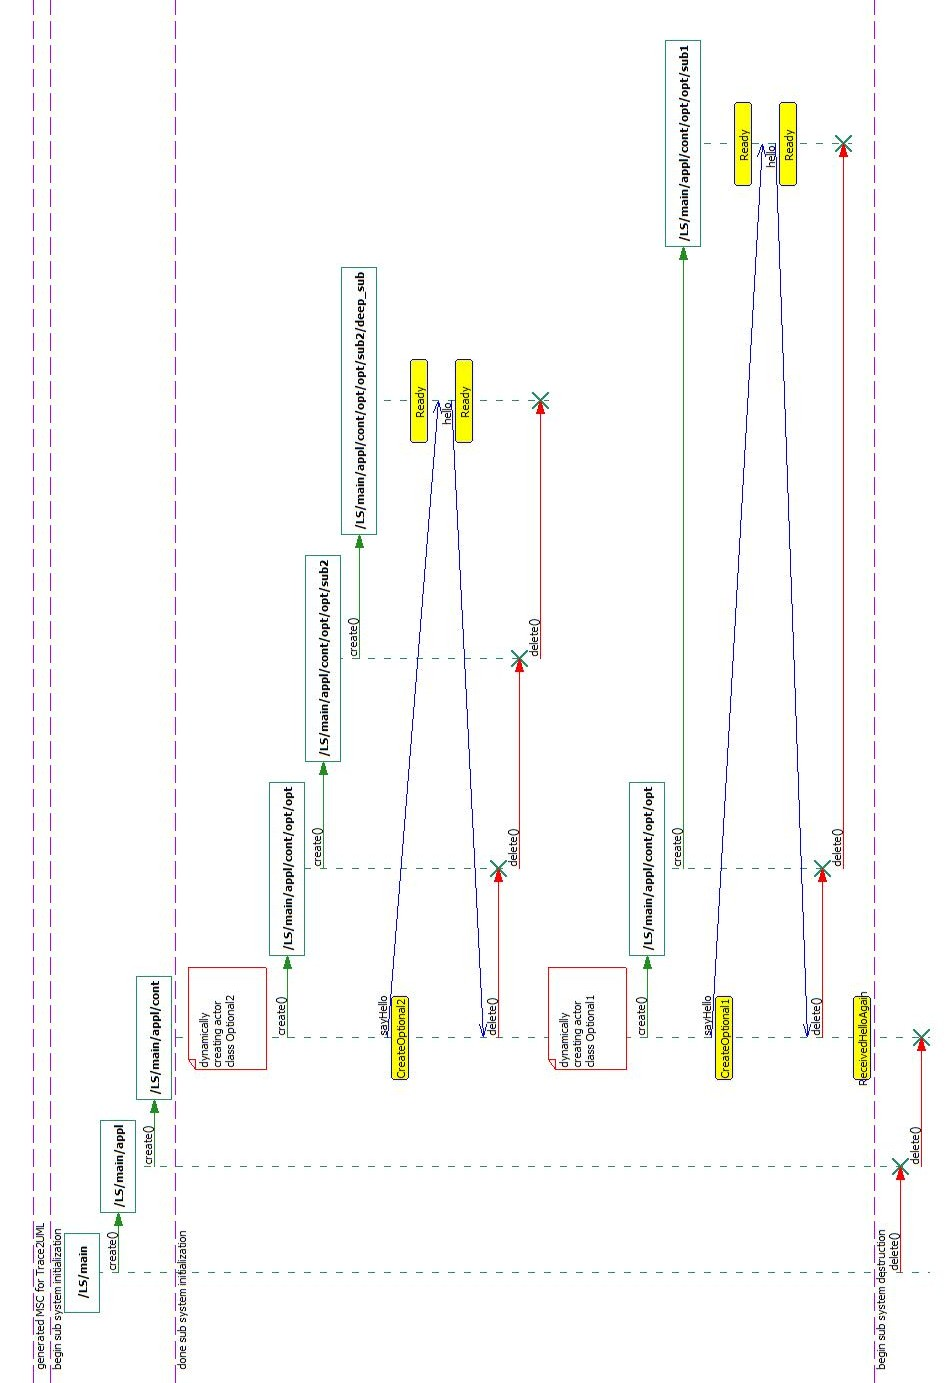
\includegraphics[scale=0.45]{images/039-DynAct1-MSC.jpg}
\caption{Sequence diagram of Dynamic Actors Example 1}
\label{fig:dynact1_msc}
\end{figure}

\subsubsection{Noteworthy}

\begin{itemize}
\item To obtain an executable the launch configuration \texttt{gen\_DynAct1\_sys.launch} has to be executed.
In this case also the SubsystemClass \texttt{Node\_nodeRef1\_main} is generated as well as factory classes
for the valid optional actors. If \texttt{Optional} were not \texttt{abstract} then also for this class
a factory is created. However, in this class the relay port isn't connected and a request \texttt{sayHello()}
would be left without reply.
\item To generate a library the launch configuration \texttt{gen\_DynAct1.launch} has to be executed.
In this case no factory classes are generated.
\end{itemize}


\subsection{Dynamic Actors 2}

This example is contained in \texttt{model/dynamicactors2}.

\subsubsection{Purpose}

A modified version of \texttt{dynamicactors1} is used to analyze eventual memory leaks of the application.

\subsubsection{Details}

In this modified version creation and deletion of optional actors is looped.
Each loop consists of 4 steps:

\begin{enumerate}
\item create an instance of \texttt{Optional2}
\item destroy the instance
\item create an instance of \texttt{Optional1}
\item destroy the instance
\end{enumerate}

All together 600 steps are performed which corresponds to 300 creations and deletions.

The free memory is printed to the console. Also the overall execution time is measured.
After the loop is finished the heap is analyzed using \texttt{JConsole} (which is a part
of the Java6 distribution) to dump the heap and
\href{http://www.eclipse.org/mat/}{\texttt{org.eclipse.mat}} to analyze it.

The measured total execution time on a Intel Core 2 Duo at 2.66 GHz was 110 ms.
This corresponds to about 370 $\mu$s.

The result of the heap analysis for \texttt{org.eclipse.etrice.*} objects is listed in figure \ref{fig:dynact2_heap}.
The small numbers per object and the retained heap size indicate that the application has no memory leak.

\begin{figure}
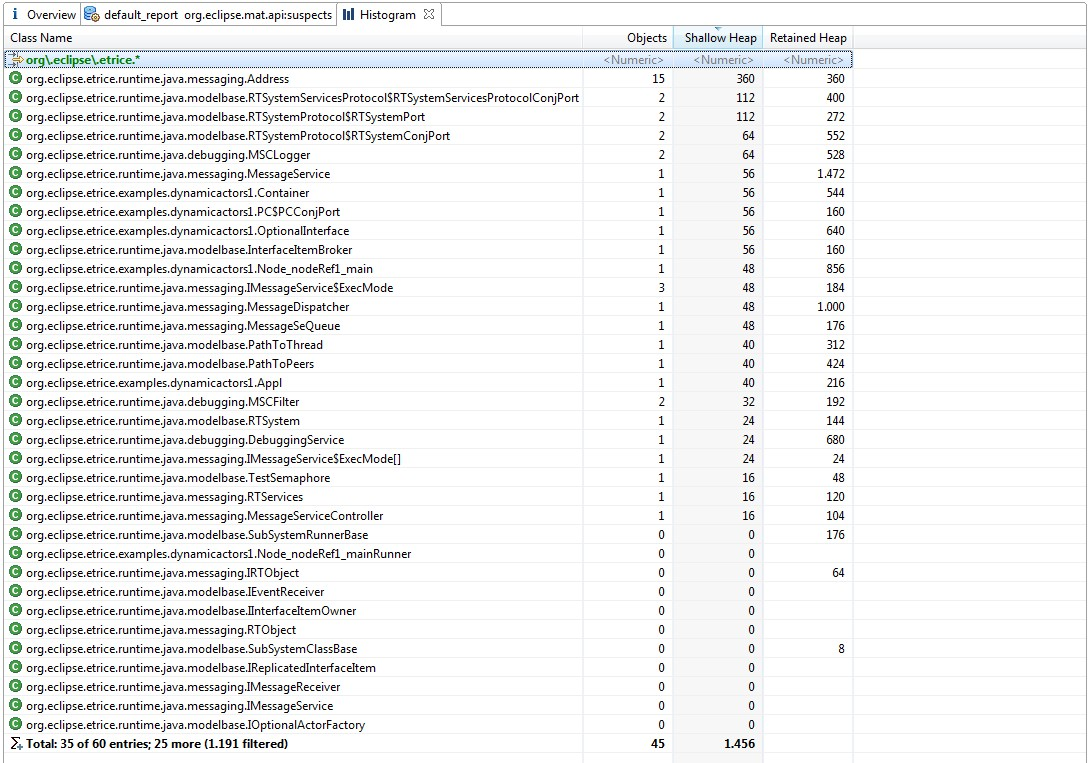
\includegraphics[scale=0.45]{images/039-DynAct2-HeapAnalysis.jpg}
\caption{Heap analysis after 600 steps}
\label{fig:dynact2_heap}
\end{figure}

\subsubsection{Noteworthy}

\begin{itemize}
\item Calling the garbage collector every time before the free memory is dumped
costs a significant amount of time and the execution time is increased to the order of seconds.
\item The measured free memory is close to constant. Only a small step is observed which wasn't analyzed further.
\end{itemize}

\subsection{Dynamic Actors 3}

This example is contained in \texttt{model/dynamicactors3}.

\subsubsection{Purpose}

The example demonstrates the usage of an optional actor array. It is shown that several actor classes
derived from the type of the optional actor reference can be created as array members.
The array members can be destroyed in arbitrary order and the array size grows and shrinks as appropriate.

\subsubsection{Details}

This example again is similar to example 1. One difference is that the (scalar) optional actor is replaced by a
replicated optional actor (or array of optional actors if you wish).
The port of the \texttt{Container} was also changed to a replicated port. All replication factors in this example
are of arbitrary multiplicity (*). The sizes vary dynamically and are unbound as far as the model is concerned.

The behavior was changed to the following:
Two instances of different classes are created as members of this array and both are deleted and one is created again.
The replicated port is used to send (broadcast) messages to the optional actors.

\subsubsection{Noteworthy}

\begin{itemize}
\item the generated MSC \texttt{main\_Async.seq} is a good illustration of the dynamic changes in the system structure
\item careful inspection of the console output reveals that objects are created and destroyed as expected
\end{itemize}

\subsection{Dynamic Actors 4}

This example is contained in \texttt{model/dynamicactors4}.

\subsubsection{Purpose}

The example demonstrates the usage of an optional actor. But here not the actor containing the optional reference
is communicating with the optional actor but one level above.

\subsubsection{Details}

The \texttt{Controller} which has a reference to the \texttt{Container} is asking the latter
for the creation of the dynamic actor. When it receives \texttt{ok()} it is requesting \texttt{sayHello()}
from the newly created actor.

After the \texttt{Controller} receives \texttt{hello()} it tells the \texttt{Container} to create another
actor which fails because the old one is still in place.

\subsubsection{Noteworthy}

\begin{itemize}
\item the generated MSC \texttt{main\_Async.seq} is a good illustration of the dynamic changes in the system structure
\end{itemize}

\subsection{Dynamic Actors 5}

This example is contained in \texttt{model/dynamicactors5}.

\subsubsection{Purpose}

The example shows that the optional actor can not only have relay ports but also external end ports.

\subsubsection{Details}

This simple example just shows that the optional actor may directly handle inbound messages by using an
external end port rather than the relay port of the previous examples.

\subsubsection{Noteworthy}

\begin{itemize}
\item the generated MSC \texttt{main\_Async.seq} is a good illustration of the dynamic changes in the system structure
\end{itemize}

\subsection{Dynamic Actors 6}

This example is contained in \texttt{model/dynamicactors6}.

\subsubsection{Purpose}

The example demonstrates the use of nested dynamic actors.

\subsubsection{Details}

In this example the dynamically created actor \texttt{Optional2} has again an optional reference two levels down in its hierarchy.
On creation it immediately creates a nested dynamic actor of class \texttt{Optional1} which is sending \texttt{hello()} back
to the outer \texttt{Container}.

\subsubsection{Noteworthy}

\begin{itemize}
\item the generated MSC \texttt{main\_Async.seq} is a good illustration of the dynamic changes in the system structure
\item when a dynamic actor is created its structure is there immediately and all ports are connected. But the initial transition
is executed asynchronously. So after the outer dynamic actor is created the port of the \texttt{Container} is not yet connected
because the initial transition which is responsible for the creation of the inner dynamic actor wasn't executed yet.
So a message sent from this port directly after creation of the outer dynamic actor would get lost.
\end{itemize}

\subsection{Dynamic Actors 7}

This example is contained in \texttt{model/dynamicactors7}.

\subsubsection{Purpose}

The example demonstrates the use of communication between two optional actors.

\subsubsection{Details}

In this example two sub trees of dynamic actors are created. The container is sending a message to one of them which is forwarding
it to the other one which in turn is replying back to the container.

\subsubsection{Noteworthy}

\begin{itemize}
\item the generated MSC \texttt{main\_Async.seq} is a good illustration of the dynamic changes in the system structure
\end{itemize}

\subsection{Dynamic Actors 8}

This example is contained in \texttt{model/dynamicactors8}.

\subsubsection{Purpose}

The example demonstrates the use of the persistence interface for dynamic actors.

\subsubsection{Details}

Dynamic actors can be persisted and restored. To this end the user has to pass an \texttt{java.io.ObjectOutput} to
the creation method (\texttt{createOptionalActor()}) and an \texttt{java.io.ObjectInput} to the deletion method (\texttt{destroyOptionalActor()}).

The code generation has to be invoked with the \texttt{-persistable} (e.g. by setting the 'generate persistence interface' flag in the Java Generator tab
of the launch configuration). This lets the generator implement the \texttt{IPersistable} interface for actor classes.

The example adds a manually coded very simple \texttt{FilePersistor} with four static methods for creation and deletion of scalar and replicated
dynamic actors.

The \texttt{Container} class first creates an optional actor of type \texttt{Optional1} in the scalar reference \texttt{opt}.
Then messages are sent to this actor instance which lead to some state changes. Finally it is saved and destroyed.
Now another actor class is instantiated in the same actor reference and also destroyed. Then the first instance is loaded from file.
It directly starts in the state it had when it was saved. The second part of the example loads copies of the two
instances created in the beginning into the \texttt{optarr} reference.

\subsubsection{Noteworthy}

\begin{itemize}
\item the generated MSC \texttt{main\_Async.seq} is a good illustration of the dynamic changes in the system structure
\end{itemize}

\subsection{Dynamic Actors 9}

This example is contained in \texttt{model/dynamicactors9}.

\subsubsection{Purpose}

The example demonstrates the use of SAPs in dynamic actors.

\subsubsection{Details}

This simple example re-uses the PingPong tutorial. The static part of the system introduces a \texttt{TimingService} as SPP
and the \texttt{Receiver} embedded in the optional part uses a SAP of this protocol.

The sub system during initialization adds broker ports to the optional actor interface that are connected to all available
services.

On the other hand the factory for the optional actor maps SAPs to those broker ports.

\subsubsection{Noteworthy}

\begin{itemize}
\item \emph{Caution:} currently the generator informs about unsatisfied services in dynamic actors. But it is still possible to create such an
instance. The consequence is an unbound SAP
\end{itemize}
